\documentclass{article}

% if you need to pass options to natbib, use, e.g.:
% \PassOptionsToPackage{numbers, compress}{natbib}
% before loading nips_2016
%
% to avoid loading the natbib package, add option nonatbib:
% \usepackage[nonatbib]{nips_2016}

\usepackage{nips_2016}

% to compile a camera-ready version, add the [final] option, e.g.:
% \usepackage[final]{nips_2016}

\usepackage[utf8]{inputenc} % allow utf-8 input
\usepackage[T1]{fontenc}    % use 8-bit T1 fonts
\usepackage{hyperref}       % hyperlinks
\usepackage{url}            % simple URL typesetting
\usepackage{booktabs}       % professional-quality tables
\usepackage{amsfonts}       % blackboard math symbols
\usepackage{nicefrac}       % compact symbols for 1/2, etc.
\usepackage{microtype}      % microtypography
\usepackage{graphicx}
\usepackage{natbib}
\usepackage{amsmath}
\usepackage{graphicx}
\usepackage{subfig}

\title{Subcellular Localization Patterns Classification with Active Learning}

% The \author macro works with any number of authors. There are two
% commands used to separate the names and addresses of multiple
% authors: \And and \AND.
%
% Using \And between authors leaves it to LaTeX to determine where to
% break the lines. Using \AND forces a line break at that point. So,
% if LaTeX puts 3 of 4 authors names on the first line, and the last
% on the second line, try using \AND instead of \And before the third
% author name.

\author{
  Xupeng Tong\\
  Computational Biology Department\\
  Carnegie Mellon University\\
  \texttt{xtong@andrew.cmu.edu} \\
}

\begin{document}
% \nipsfinalcopy is no longer used

\section{generalized Factorization Machine}

\begin{figure}
\begin{tabular}{cc}
  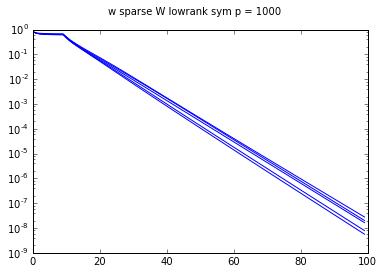
\includegraphics[width=65mm]{gfm_plots/w_sparse_W_lowrank_sym.png} &   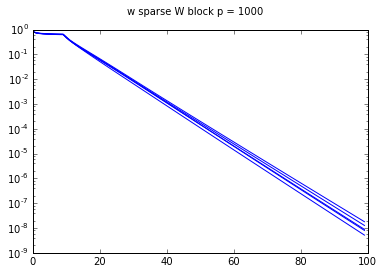
\includegraphics[width=65mm]{gfm_plots/w_sparse_W_block} \\
(a) w sparse W low rank and symmetric & (b) w sparse W block \\[6pt]
 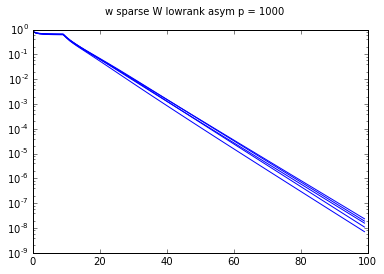
\includegraphics[width=65mm]{gfm_plots/w_sparse_W_lowrank_asym} &   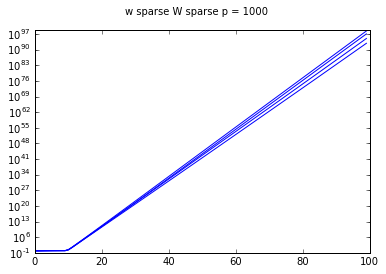
\includegraphics[width=65mm]{gfm_plots/w_sparse_W_lowrank_sparse} \\
(c) w sparse W low rank and asymmetric & (d) w sparse W sparse \\[6pt]
\end{tabular}
\caption{caption}
\end{figure}

We observed that when gFM is dealing with $W$ that has a sparse structure, the error rate on the training data explodes, probably because its updating through the sequence of estimation does not necessarily require the error change in a descent manner.

Similarly, choosing the rank $k$ of the training data as close to the original rank $k$ in is important. As it determines the initialization of $U$ in the algorithm described, estimating $k$ by a large number would almost certainly cause the error rate explodes. The updating rule used in this algorithm is highly sensitive to apriori knowledge about the structure though it can't be easily estimated without certain domain knowledges.

The learning rate, as used to describe the algorithm of gFM, differs from the learning rate we know from algorithms we familiar with from the first order or second order algorithms. Instead, they use learning rate here to denote the degree a single estimation can learn. We tried setting up different learning rate and found that within a certain small window of learning rate, the error rate can decrease linearly with a considerable rate, while with a slightly larger learning rate, linearly increased error rate can be observed.

Generally, generalized factorization machine and its associated algorithm bridges the theoretical gap between the matrix sensing problem and the factorization machine. The problem it deals with is naturally non-convex which means the conventional gradient descent framework can hardly achieve a global convergence. It is proved that the algorithm they proposed can achieve a linear convergence rate and it is also shown in our experiment. However, we found it to be tricky to fine tune the parameters such as learning rate and the rank $k$ before applying this algorithm, which makes it somewhat impractical in a real world setting.


\end{document}
